\newpage
\section{Chapter 2}

\begin{figure}[H]
	\centering
	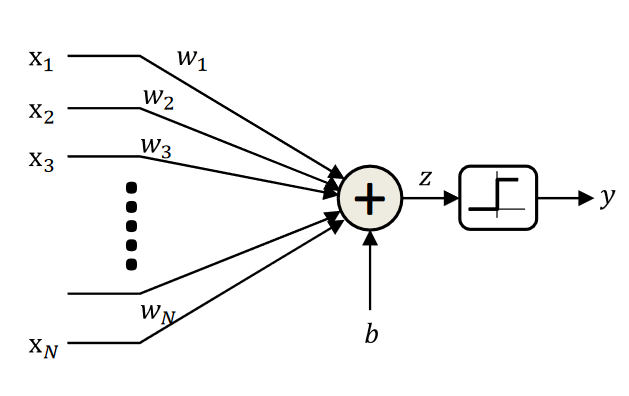
\includegraphics[width=0.5\textwidth]{2_perceptron}
\end{figure}

\hfill\break
Each individual neurons can be represented as a threshold unit.
\begin{itemize}
	\item It fires if the affine function of inputs is positive.
	\item The bias value is the negative of threshold $T$.
\end{itemize} 

\begin{align*}
	z &= \sum_{i}w_ix_i + b \\
	y &= 
\begin{cases} 
	1, & \text{if } z \geq 0 \\
	0, & \text{else }
\end{cases}
\end{align*}

\hfill\break
Once we can represent the neuron in this manner, we can modify the activation threshold function to something different such as:
\begin{itemize}
	\item We define \textbf{activation function} as the function that acts on the weighted combination of inputs and bias.
	 
\end{itemize}
\paragraph{Soft Perceptron (Logistic)}
A squashing function instead of a threshold at the output. This way the output goes rather smooth from $0$ to $1$.
\begin{align*}
	z &= \sum_{i}w_ix_i + b \\
	y &= \frac{1}{1 + \exp (-z)}
\end{align*}

\hfill\break
We can also replace the activation function with other mathematical function such as $\tanh$, $\text{softplus}$ and $\text{rectifier}$.

\subsection{Multi-layer Perceptron}
MLP is a network of perceptrons as the perceptrons of current layer are fed to other perceptrons on the next layer.

\paragraph{Deep Structures}
In any directed graph with input source nodes and output sink nodes, ``depth'' is the length of the longest path from a source to a sink.
\begin{itemize}
	\item A ``source'' node in a directed graph is a node that has only outgoing edges.
	\item A ``sink'' node is a node that has only incoming edges.
\end{itemize}

\hfill\break
This is an example of depth 2 graph.
\begin{figure}[H]
	\centering
	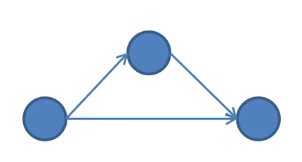
\includegraphics[width=0.4\textwidth]{2_2depth}
\end{figure}

\hfill\break
This is an example of depth 3 graph.
\begin{figure}[H]
	\centering
	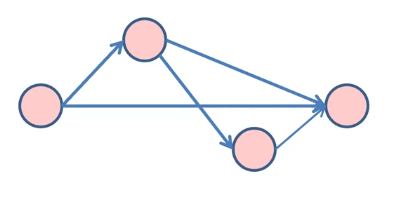
\includegraphics[width=0.4\textwidth]{2_3depth}
\end{figure}

\hfill\break
In multilayer perceptron, a network is considered ``deep'' if the depth of the output neurons is greater than $2$.

\subsection{Layer}
Layer is a set of neurons that are all at the same depth  with respect to the input (sink). This would imply that the ``depth'' of the layer is the depth of the neurons in the layer with respect to the input.

\begin{figure}[H]
	\centering
	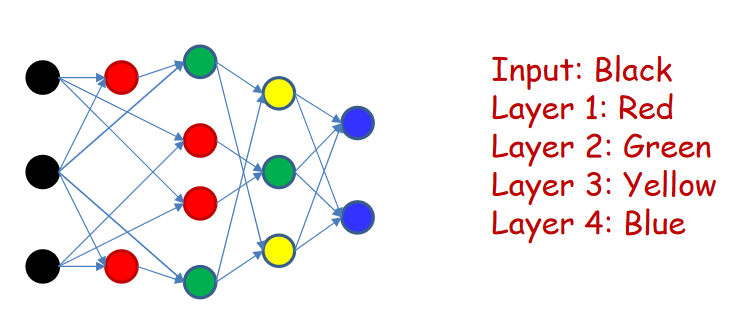
\includegraphics[width=0.75\textwidth]{2_layer}
\end{figure}

\hfill\break
In multi-layered perceptron:
\begin{itemize}
	\item Inputs are real or Boolean stimuli.
	\item Outputs are real or Boolean values.
	\item It can compose both Boolean and real-valued functions.
	\item We can have multiple outputs for a single input.
\end{itemize}

\subsection{MLP as universal Boolean functions.}
We are already aware with perceptron capability as a Boolean gate as it can model any simple binary Boolean gate (OR, AND \& NOT).

\begin{figure}[H]
	\centering
	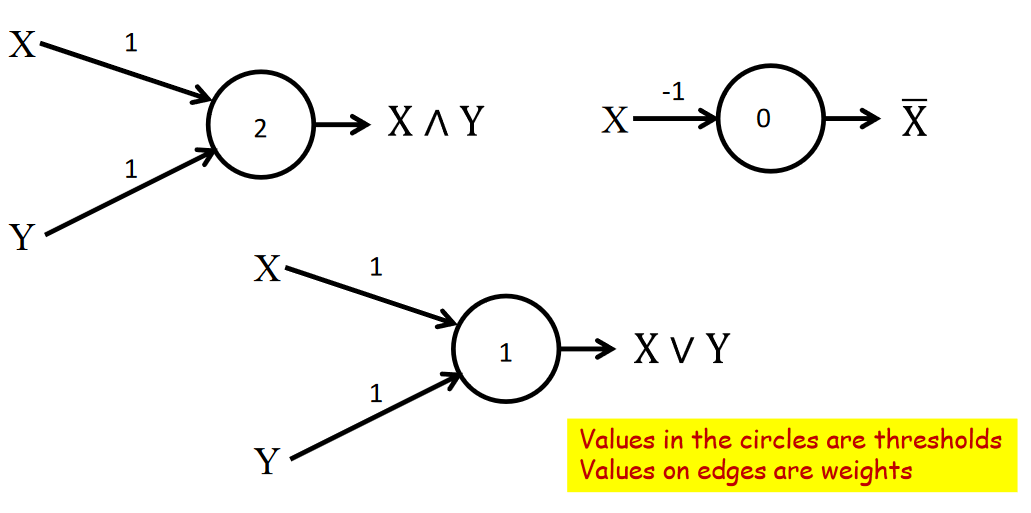
\includegraphics[width=\textwidth]{2_boolean_gate}
\end{figure}

\hfill\break
It also enables us to compose a much more complex network, for example a universal AND gate where the network is only fired if every input fed to the network is true.

\begin{figure}[H]
	\centering
	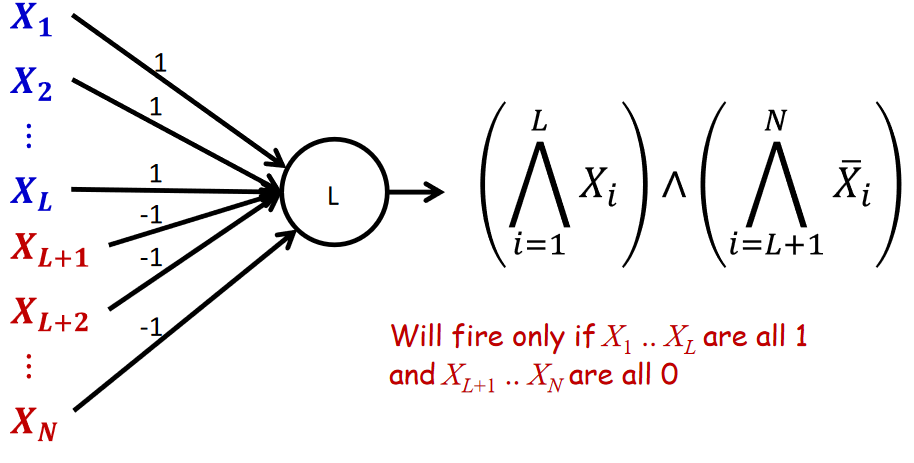
\includegraphics[width=0.5\textwidth]{2_universal_and}
\end{figure}

\subsection{Summary}
With enough ``depth'':
\begin{itemize}
	\item MLP as universal Boolean functions.
	\item MLP as universal classifiers.
	\item MLP as universal approximators.
\end{itemize}
